\documentclass[border={0.1cm 0.1cm 0.1cm 0.1cm}]{standalone}  %E,S,W,N

\usepackage{amssymb}
\usepackage{amsmath}
\usepackage{tikz}
\usetikzlibrary{calc}	%for centerarc

\def\centerarc[#1](#2)(#3:#4:#5) {\draw[#1] ($(#2)+({#5*cos(#3)},{#5*sin(#3)})$) arc (#3:#4:#5);}

%by James M. Dow -- https://twitter.com/jmatthiasdow/status/1401892108705927168

\begin{document}
	
	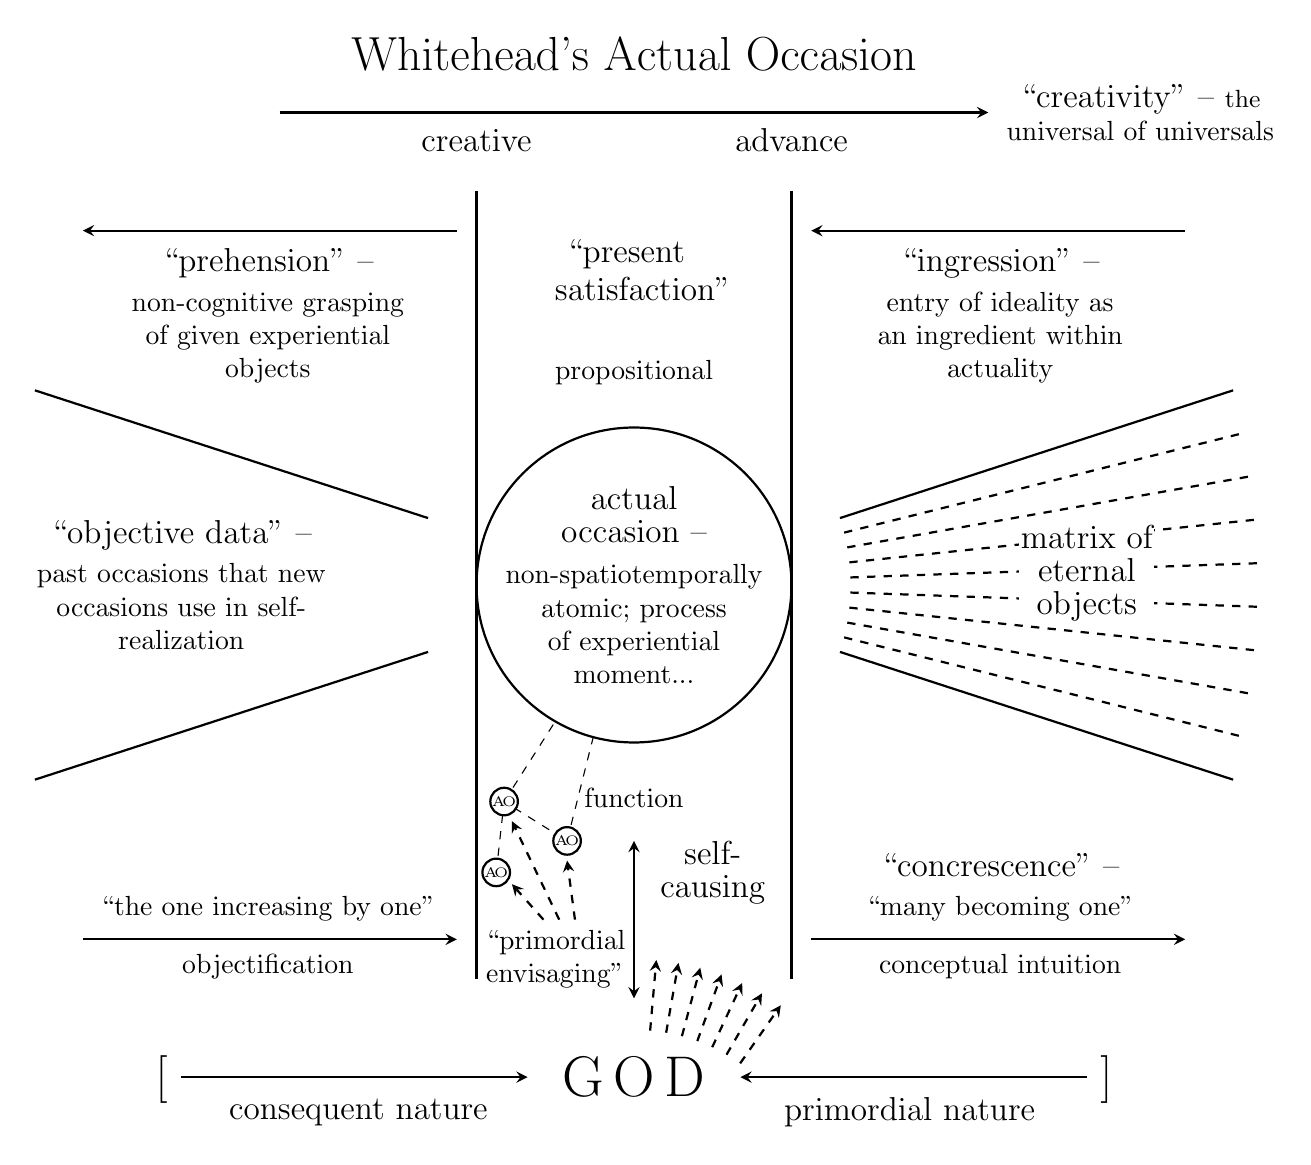
\begin{tikzpicture}[thick]
	%MIDDLE CIRCLE
	\draw (0,0) circle (2cm);
	\node[align=center] at (0,0) {\large actual \\ \large occasion -- \\[1mm] non-spatiotemporally \\ atomic; process \\ of experiential \\ moment...};
	\centerarc[->,>=stealth](0,0)(40:140:2.5)
	\centerarc[->,>=stealth,dashed](0,0)(145:215:2.5)
	\centerarc[->,>=stealth](0,0)(220:320:2.5)
	\centerarc[->,>=stealth,dashed](0,0)(325:395:2.5)
	\node at (0,2.7) {propositional};
	\node at (0,-2.7) {function};
	\node[align=center] at (0,4) {\large $\!\!\!$``present \\[0.5mm] \large $\;\;$satisfaction''};
	
	%LINES
	\draw (-2,-5)--(-2,5);	%horizontal left
	\draw (2,-5)--(2,5);	%horizontal right
	%
	\draw[->,>=stealth] (-2.25,4.5)--(-7,4.5);
	\node[align=center,below] at (-4.65,4.4) {\large ``prehension'' -- \\[0.75mm] non-cognitive grasping \\ of given experiential \\ objects};
	%
	\draw[->,>=stealth] (7,4.5)--(2.25,4.5);
	\node[align=center,below] at (4.65,4.4) {\large ``ingression'' -- \\[0.75mm] entry of ideality as \\ an ingredient within \\ actuality};
	%
	\draw[->,>=stealth] (-7,-4.5)--(-2.25,-4.5);
	%\node[align=center,above] at (-4.65,-4.4) {\large ``primordial envisaging'' -- \\[0.75mm] ``the one increasing by one''};
	\node[align=center,above] at (-4.65,-4.4) {``the one increasing by one''};
	\node at (-4.65,-4.85) {objectification};
	%
	\draw[->,>=stealth] (2.25,-4.5)--(7,-4.5);
	\node[align=center,above] at (4.65,-4.4) {\large ``concrescence'' -- \\[0.75mm] ``many becoming one''};
	\node at (4.65,-4.85) {conceptual intuition};
	
	%TOP LABELS
	\node at (0,6.75) {\LARGE Whitehead's Actual Occasion};
	\draw[->,>=stealth] (-4.5,6)--(4.5,6);
	\node at (-2,5.65) {\large creative};
	\node at ( 2,5.65) {\large advance};
	\node[align=center,right] at (4.6,6) {\large ``creativity'' -- {\small the} \\ universal of universals};
	
	%SIDE PARTS
	\node[align=center] at (-5.75,0) {\large ``objective data'' -- \\[0.75mm] past occasions that new \\ occasions use in self- \\ realization};
	%
	\draw ({2.75*cos(18)},{2.75*sin(18)})--({8*cos(18)},{8*sin(18)});
	\draw ({2.75*cos(-18)},{2.75*sin(-18)})--({8*cos(-18)},{8*sin(-18)});
	%
	\draw ({2.75*cos(180-18)},{2.75*sin(180-18)})--({8*cos(180-18)},{8*sin(180-18)});
	\draw ({2.75*cos(180+18)},{2.75*sin(180+18)})--({8*cos(180+18)},{8*sin(180+18)});
	%
	\foreach \i in {1,...,8} \draw[dashed] ({2.75*cos(18-4*\i)},{2.75*sin(18-4*\i)})--({8*cos(18-4*\i)},{8*sin(18-4*\i)});
	%
	\node[align=center,fill=white,inner sep=0.5] at (5.75,0.15) {\large matrix of \\ \large eternal \\ \large objects};
	
	%UNDER CIRCLE
	\draw[<->,>=stealth] (0,-3.25)--(0,-5.25);
	\node[align=center] at (1,-3.65) {\large self- \\\large causing};
	%
	\draw[dashed,thin] (-1.65,-2.75)--({2*cos(240)},{2*sin(240)});
	\draw[dashed,thin] (-0.85,-3.25)--({2*cos(255)},{2*sin(255)});
	\draw[dashed,thin] (-1.75,-3.65)--(-1.65,-2.75)--(-0.85,-3.25);
	\draw[fill=white] (-1.65,-2.75) circle (0.175cm) node {\tiny A$\!$O};
	\draw[fill=white] (-0.85,-3.25) circle (0.175cm) node {\tiny A$\!$O};
	\draw[fill=white] (-1.75,-3.65) circle (0.175cm) node {\tiny A$\!$O};
	%
	\draw[->,>=stealth,dashed] (-0.75,-4.25)--(-0.85+0.0,-3.25-0.25);
	\draw[->,>=stealth,dashed] (-0.95,-4.25)--(-1.65+0.1,-2.75-0.25);
	\draw[->,>=stealth,dashed] (-1.15,-4.25)--(-1.75+0.2,-3.65-0.15);
	%
	\node[align=center] at (-1,-4.75) {``primordial \\ envisaging''};
	
	%BOTTOM PART
	\node at (0,-6.25) {\huge G$\,$O$\,$D};
	\draw[->,>=stealth] (-5.75,-6.25)--(-1.35,-6.25);
	\node at (-3.5,-6.7) {\large consequent nature};
	\draw[->,>=stealth] (5.75,-6.25)--(1.35,-6.25);
	\node at (3.5,-6.7) {\large primordial nature};
	\node at (-6,-6.28) {\LARGE [};
	\node at ( 6,-6.28) {\LARGE ]};
	\foreach \i in {1,...,7} \draw[->,>=stealth,dashed] ({2.35*cos(90-5*\i)},{-8+2.35*sin(90-5*\i)})--({3.25*cos(90-5*\i)},{-8+3.25*sin(90-5*\i)});
	\end{tikzpicture}
	
\end{document}